    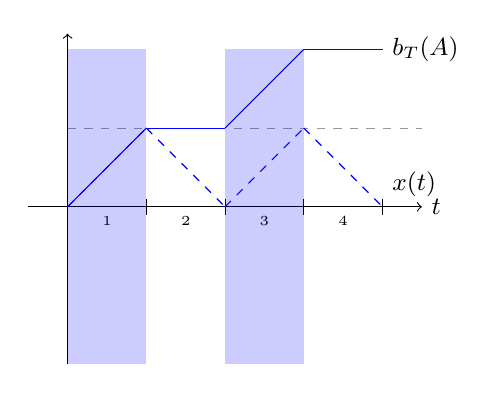
\begin{tikzpicture}
        % Draw x-axis

        \draw[->] (-.5,0) -- (4.5,0) node[right, font=\small] {$t$};
        \draw[dashed, opacity=0.4] (0,1) -- (4.5,1);
        % \node at (0, 1) [left, font=\tiny] {$\overline{x}$};
        % Draw y-axis
        \draw[->] (0,-2) -- (0,2.2);

        % \node at (0, 2) [left, font=\tiny] {$x(t)$};

        % Add ticks on x-axis
        \foreach \x in {1,2,3,4}
            \draw (\x,0.1) -- (\x,-0.1);
        
        \foreach \x in {1,2,3,4}
            \draw (\x - 0.5 ,0) -- (\x-0.5,-0) node[below, font=\tiny] {\x};

        % Shade a vertical region
        \foreach \x in {1, 3}
            \fill[blue, opacity=0.2] (\x-1,-2) rectangle (\x,2);
        \draw[blue, -] (0, 0) -- (1, 1);\draw[blue] (1, 1) -- (2, 1);\draw[blue, -] (2, 1) -- (3, 2);\draw[blue] (3, 2) -- (4, 2);\node at (4, 2) [right, font=\small] {$b_T(A)$};
        \draw[dashed, blue] (0, 0) -- (1, 1);\draw[dashed, blue] (1, 1) -- (2, 0);\draw[dashed, blue] (2, 0) -- (3, 1);\draw[dashed, blue] (3, 1) -- (4, 0);\node at(4, 0) [above right, font=\small] {$x(t)$};

            
    \end{tikzpicture}

    